\documentclass[addpoints,12pt]{exam}

%\usepackage{newtxtext,newtxmath} % times new roman font
\usepackage{url}
\usepackage[dvipsnames]{xcolor}
\usepackage{enumitem}

\usepackage{bm,mathtools}
\DeclarePairedDelimiter\ceil{\lceil}{\rceil}

\usepackage{tikz}
\usetikzlibrary{shapes}

\usepackage{titling}
\setlength{\droptitle}{-6em}

\title{Midterm Exam \#1\\[0.25em]
\large CSC 485C/586C: Data Management on Modern Computer Architectures\\
Friday 14 February 2020, 10.35-11.20}
\date{}

\begin{document}
\maketitle

\vspace{-6.5em}
{\centering
  \hspace{0.05\textwidth}
  \parbox{0.6\textwidth}{%
    Name:\enspace\hrulefill
  }\hspace{2em}
  \parbox{0.25\textwidth}{%
    V00\enspace\hrulefill
  }
}

\bigskip
\printanswers
\begin{questions}
 \question Please explain the following concepts in 1-3 sentences and/or code snippets and/or a small illustration.  An excellent answer does not have to be long, just precise.\\{\em Guide: 2 minutes each} 

 \medskip
 
 \begin{parts}
   \part[1] Bad Speculation
     \begin{solution}[6em]
Branch prediction gone wrong. Instructions were executed out-of-order on a branch for which the condition had not yet been evaluated, and it turned out that the result of the condition is that those instructions should not have been executed, after all (and must be undone!)
     \end{solution}
   
   \part[1] Cold Data
     \begin{solution}[6em]
Data that isn't used very often (relative to ``hot data''). (Important because it pollutes cache, effectively shrinking it.)
     \end{solution}
   
   \part[1] Latency
     \begin{solution}[6em]
The wait for something to happen, usually measured in cycles. E.g., a memory latency of 240 or an instruction latency of 1 cycle means that one must wait 240 cycles or 1 cycle, respectively, for the memory load or instruction to complete.
     \end{solution}
   
   \part[1] Locality of Reference
     \begin{solution}[6em]
Accessing (i.e., referencing) data that is nearby what you just accessed.
     \end{solution}
   
   \part[1] Memory-Bound
     \begin{solution}[6em]
The bottleneck of the application is the memory subsystem (either latencies or bandwidth)
     \end{solution}
 \end{parts}
 
 \newpage
 \question You have a contiguously laid out, sequential linked list in which each node of the linked list is defined as follows:

\begin{verbatim}
struct Node
{
    Node *next;
    char padding[ npad ]; // npad is a constant defined elsewhere
};
\end{verbatim}

Answer the following questions that analyse this figure below (taken from Drepper):\\
{\em Guide: 10 min total}

\hspace{0.2\textwidth}\parbox{0.6\textwidth}{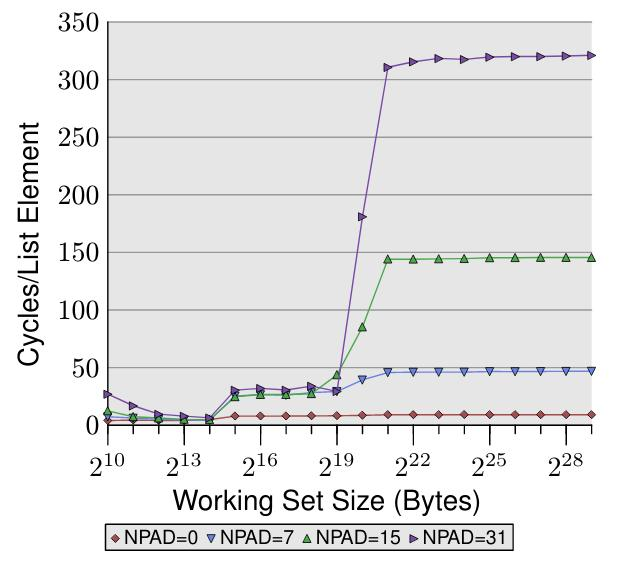
\includegraphics[ scale = 0.5]{fig/drepper-wss.jpg}}


   \begin{parts}
       \part[2] What does the shape of the trendlines indicate?
           \begin{solution}[5em]

Full marks should indicate at least two of the following:
\begin{itemize}
  \item The step-function shape reflects the abrupt cost of no longer being cache-resident
  \item The three separate plateaus reflect the working set size being fully L1-, L2-, and L3-cache-resident, respectively
  \item The $x$-value at which the curve jumps is approximately the size of the cache
\end{itemize}
           \end{solution}

       \newpage
       \part[2] Why does the curve corresponding to \texttt{npad=0} appear not to have the same shape as the other curves?
           \begin{solution}[5em]

Full marks should indicate at least two of the following:
\begin{itemize}
  \item It {\em does} have the same shape as the other \texttt{npad} values, but the difference is dwarfed by a $y$-axis large enough to capture the worst latencies for \texttt{npad=31}
  \item Because a pointer is only 8B and a cache line is 64B, we retrieve 8 nodes per cache line when there is no padding; locality is excellent as we use every value on every cache line.
  \item The prefetcher minimises the memory latencies
\end{itemize}
           \end{solution}

       \part[2] What is the overall message (a.k.a., purpose, or significance) of the plot?
           \begin{solution}[5em]

({\em specific responses may vary but should be similar})\\
The paper is called ``What Every Programmer Should Know About Memory.'' This plot illustrates the cost of not controlling your "working set size", i.e., because of poor locality and/or unoptimised data structures. By using four separate trendlines, it especially indicates the cost of having consecutive data accesses increasingly far apart (i.e., having a lot of ``cold data'').
           \end{solution}
   \end{parts}
 
 
  \question[8] A ``Palentine's Card'' is a warm greeting card that one gives to a friend on 14 February. Below we have a data structure to define a set of Palentine's Cards and an algorithm to count how many pairs have the same sender {\em and} recipient, i.e., cases where one person gave multiple cards to the same pal. Sadly, the implementation suffers from poor cache performance. Rewrite both the implementation and the data structures to optimise cache performance. (Pseudocode or annotations is fine; proper syntax is not evaluated, so long as the intent is clear.)\\
{\em Guide: 15 min}
  
   \bigskip
    \begin{minipage}{.4\textwidth}
      \begin{verbatim}
struct palentine
{
  std::string sender_name;
  std::string recipient_name;
  std::string message;
};

// overload == for palentine
bool operator == ( /*...*/ )
{
    // return true if both sender
    // and recipient match
}

std::vector< palentine > cards;
      \end{verbatim}
    \end{minipage}
    \hfill
    \begin{minipage}{.5\textwidth}
      \begin{verbatim}
template < typename T >
auto num_matching_cards( T const& cards )
{
    auto const n = cards.size();
    auto num_matches = 0llu;

    for( auto i = 0u; i < n; ++i )
    {
        for( auto j = i + 1; j < n; ++j )
        {
            if( cards[ i ] == cards[ j ] )
                ++num_matches;
        }
    }
    return num_matches;
};
      \end{verbatim}
    \end{minipage}
    

      \begin{solution}[15em]

Full marks for:
\begin{itemize}
  \item Increasing spatial locality by decreasing working set size by:
    \begin{itemize}
      \item converting AoS to SoA by taking the ``cold'' \texttt{std::string message} out of the main struct
      \item replacing the \texttt{std::string *\_name}'s with pointers to a struct containing the names (preferably organised in a vector)
    \end{itemize}
  \item Increasing temporal locality by:
    \begin{itemize}
      \item Tiling the outer loop over $i$
    \end{itemize}
  \item Other useful optimisations in lieu of those above
\end{itemize}
A bonus mark will be given if the pointers to the structs are moreover replaced by an index into the array of person structs, clarifying the assumptions about the number of distinct persons. This can decrease the size of the hot data even further.

   \bigskip
    \begin{minipage}{.35\textwidth}
      \begin{verbatim}
struct person
{
  std::string name;
};

std::vector< person > people;

struct header
{
  uint32_t sender_id;
  uint32_t recipient_id;
};

struct cards
{
  using namespace std;

  vector< header > headers;
  vector< string > messages;

  auto size() const
  {
    return headers.size();
  }
};
      \end{verbatim}
    \end{minipage}
    \hfill
    \begin{minipage}{.6\textwidth}
      \begin{verbatim}
template < typename T >
auto num_matching_cards( T const& cards )
{
    auto const n = cards.size();
    auto const tile_size = 4u;
    auto num_matches = 0llu;

    for(auto i=0u; i<n; i += tile_size )
    {
      for(auto j=i+1; j < n; ++j)
      {
        for(auto k=0u; k < tile_size; ++k)
        {
          if( cards.headers[ i ]
           == cards.headers[ j ] )
            ++num_matches;
        }
      }
    }
    return num_matches;
};



      \end{verbatim}
    \end{minipage}

      \end{solution}
    
    \question[2] How would you verify that your optimisations to \texttt{num\_matching\_cards()} improved cache performance?\\
{\em Guide: 5 min}
      
      \begin{solution}[5em]
We should measure both:
\begin{itemize}
  \item The total number of loads from each level of cache. A smaller working set size should require reading less data overall
  \item The total number and/or percentage of loads that miss (especially that cause a stall) each level of cache, indicating improved locality
\end{itemize}
      \end{solution}

    \newpage
    \question Answer the following two questions on the data structure below:\\
{\em Guide: 5 min}

\begin{verbatim}
struct box_of_chocolates
{
    uint16_t num_milk_chocolates;
    uint16_t num_dark_chocolates;
    uint8_t  num_white_chocolates;
    uint32_t box_size; // volume in cubic millimeters
};
\end{verbatim}

      \begin{parts}
         \part[2] Considering alignment, how would you change this struct without changing any data types so that your working set size was reduced?\\
      
      \begin{solution}[8em]

({\em Note that this question contained a typo. The milk chocolates were supposed to only use 1 byte. Obviously I had a hard time convincing myself that $2^8$ milk chocolates are quite enough\ldots})

\medskip
With 2B of milk chocolates, the struct above contains 3B of padding between the white chocolates and the box size; thus the total struct uses 12B. With 1B of milk chocolates, there is also another 1B of padding between the milk and dark chocolates, so it still requires 12B.

\medskip
Ordering the fields descending by the size of their data types removes the need for padding. With 2B of milk chocolates, this still requires 9B which will round up to 12B (to fit a ``word''); with 1B of milk chocolates, this now requires 8B, which decreases the working set size by 33\%.
      \end{solution}

         \part[1] How would you verify that your changes had reduced the working set size?\\
      
      \begin{solution}[5em]
Measure it directly. There are many ways to do this, but the simplest is to call `sizeof()` inside a \texttt{c++} application.

\medskip
You could also check the assembly that is generated, print a bunch of them to a binary file and measure the file size, or, in a more indirect sense, measure if there was a speed up in running time.
      \end{solution}
    
      \end{parts}
\end{questions}

\vfill
\begin{minipage}{.2\textwidth}\hphantom{xxxxxxxxxxx}\end{minipage}
\gradetable[h][questions]

\end{document}
